\NeedsTeXFormat{LaTeX2e}

% Font size = 10, DIV = 11 to reduce waste of space %
\documentclass[a4paper,10pt
headsepline,           % Linie zw. Kopfzeile und Text
doubleside,            % doppelseitig
pointlessnumbers,      % keine Punkte nach den letzten Ziffern in Überschriften
bibtotoc,              % LV im IV
%DIV=15,               % Satzspiegel auf 15er Raster, schmalere Ränder   
BCOR15mm,               % Bindekorrektur
leqno					% equation numbers to the left
% fleqn
%,draft
]{scrbook}
\KOMAoptions{DIV=11} % Neuberechnung Satzspiegel nach Laden von Paket helvet

% be able to include real vector graphics in thesis. You need inkscape installed and your pdflatex command must be called with --shell-escape for this to work.
% TeXstudio: Options → Configure → Commands → pdflatex = pdflatex -synctex=1 -interaction=nonstopmode --shell-escape %.tex
% inkscape=newer to avoid re-export if nothing has changed in the svg. inkscapelatex=false for not using latex to render text (which in turn messes up all text in image). inkscapearea = page so that the SVG size is respected and borders in the SVG are not cut off
%\usepackage[inkscape=newer, inkscapelatex=false, inkscapearea=page]{svg} 

\pagestyle{headings}
\usepackage{blindtext}

% für Texte in deutscher Sprache
\usepackage[ngerman, USenglish]{babel}
\usepackage[utf8]{inputenc}
\usepackage[T1]{fontenc}

% enable HERE positioning %
\usepackage{float}

\usepackage{scrhack}

% Helvetica als Standard-Dokumentschrift
\usepackage[scaled]{helvet}
\renewcommand{\familydefault}{\sfdefault} 


\usepackage{graphicx}

% Literaturverzeichnis mit BibLaTeX // use Biber as Backend; dashed = false to repeat author names
\usepackage[babel]{csquotes}
\usepackage[backend=bibtex,style=ieee,dashed=false,hyperref,natbib]{biblatex}
\addbibresource{BA.bib}

% Für Tabellen mit fester Gesamtbreite und variabler Spaltenbreite
\usepackage{tabularx} 

% multirow tables
\usepackage{multirow}

% arrows in normal text, not only math
\newcommand*{\textrightarrow}{$ \rightarrow $}

\newcommand*{\textdownarrow}{$ \downarrow $}


% Besondere Schriftauszeichnungen
\usepackage{url}              % \url{http://...} in Schreibmaschinenschrift
\usepackage{color}            % zum Setzen farbigen Textes

\usepackage{setspace}         % Paket für div. Abstände, z.B. ZA
\setlength{\parindent}{0pt}   % kein linker Einzug der ersten Absatzzeile
\setlength{\parskip}{1.4ex plus 0.35ex minus 0.3ex} % Absatzabstand, leicht variabel

% Tiefe, bis zu der Überschriften in das Inhaltsverzeichnis kommen
\setcounter{tocdepth}{2}      % 3 ist Standard
\setcounter{secnumdepth}{3}   % 2 ist Standard

% don't list subsections of appendices in TOC
\usepackage{tocvsec2}


% Mathe
\usepackage{amsfonts}
\usepackage{amssymb}
%\usepackage{amsmath}
% Multilined / aligned command %
\usepackage{mathtools}

% Plots - https://www.overleaf.com/learn/latex/Pgfplots_package
\usepackage{pgfplots}

\pgfkeys{/pgf/number format/.cd,1000 sep={}}
\pgfplotsset{
	compat=newest,
	legend style={at={(0.5,-0.2)},anchor=north}, % legend to the bottom
	legend cell align={left}, % left align legend text
	ymajorgrids=true, 
	grid style=dashed,
	scaled ticks=false, % don't use 10^x notation
	tick label style={/pgf/number format/fixed},
	try min ticks=8,
	tick pos=left % no ticks at the right / top borders
}

% Landscape pages
\usepackage{pdflscape}

% diagonal boxes in table
\usepackage{diagbox}

% resume enumerate https://tex.stackexchange.com/questions/210429/how-can-a-bring-a-middle-paragraph-out-of-the-enumerate-environment
\usepackage{enumitem}

\usepackage[utf8]{inputenc}

% Pseudocode %
\usepackage[lined, algochapter, resetcount, linesnumbered]{algorithm2e}
\SetKwData{Left}{left}\SetKwData{This}{this}\SetKwData{Up}{up}
\SetKwFunction{Union}{Union}\SetKwFunction{FindCompress}{FindCompress}
\SetKwInOut{Input}{input}\SetKwInOut{Output}{output}
\SetKw{Continue}{continue}
\newcommand{\Function}[3]{
	\SetKwBlock{FunctionBlock}{function \textnormal{\textsc{#1} (\emph{#2})}}{end function}
	\FunctionBlock{#3}
}


\usepackage{hyperref, xcolor,microtype,ifthen}
% Cleveref so we don't have to write "Section \ref" each time and nameinlink so that the word "Section" also belongs to the PDF link!
\usepackage[nameinlink]{cleveref}
\usepackage{graphicx}

% used for subfigures
\usepackage{subcaption}

% used for multi-page graphics
\usepackage{caption}
\usepackage{zref-savepos}
\usepackage{dpfloat}
%\providecommand*{\zsaveposy}{\zsavepos}% support older zref-savepos

% Don't abbreviate figure crefs. Also support algorithm2e listings %

\crefname{figure}{figure}{figures}
\crefname{equation}{formula}{formulas}
\crefname{algorithm}{algorithm listing}{algorithm listings}

\creflabelformat{equation}{#2#1#3}

% Graphen und sonstige Zeichnungen
\usepackage{tikz}
\usetikzlibrary{shapes.geometric}
\usetikzlibrary{shapes.misc}
\usetikzlibrary{positioning}
\usetikzlibrary{calc}

% Layout
\usepackage[scale=0.70, marginratio={4:5, 3:4}, ignoreall, headsep=8mm]{geometry}
\setlength{\parskip}{1.4ex plus 0.35ex minus 0.3ex}
\renewcommand\arraystretch{1.3} % höhere Zeilen in Tabellen
\clubpenalty10000  % keine Schusterjungen
\widowpenalty10000 % keine Hurenkinder
\setcounter{tocdepth}{3} % Tiefe, bis zu der Überschriften in das Inhaltsverzeichnis kommen


% vertical table headers https://tex.stackexchange.com/questions/98388/how-to-make-table-with-rotated-table-headers-in-latex
\usepackage{adjustbox}
\usepackage{array}
\usepackage{booktabs}

% partial function arrow https://tex.stackexchange.com/questions/47142/how-to-tex-an-arrow-with-vertical-stroke %
\newcommand\pto{\mathrel{\ooalign{\hfil$\mapstochar\mkern5mu$\hfil\cr$\to$\cr}}}

% autorefs %
\def\sectionautorefname{section}

% Beispiele für Quellcode
\usepackage{listings}
\lstset{language=Java,
  showstringspaces=false,
  frame=single,
  numbers=left,
  basicstyle=\ttfamily,
  numberstyle=\tiny
  captionpos=b,
  numbers=left,
  basicstyle=\singlespacing\ttfamily,
  numberstyle=\smaller\ttfamily,
  tabsize=4
}

\makeatletter
\AtBeginDocument{\@ifpackageloaded{amsmath}{\@mathmargin\z@}{}}%
\makeatother

% hier Namen etc. einsetzen
\newcommand{\fullname}{Florian Lappe}
\newcommand{\email}{florian.lappe@uni-ulm.de}
\newcommand{\titel}{}
\newcommand{\untertitel}{Development and Evaluation of a Metamodel to Define Modeling Syntaxes for CouchEdit}
\newcommand{\jahr}{2020}
\newcommand{\abgabedatum}{August 2020}
%\newcommand{\abschlussarbeit}{Bachelorarbeit}
\newcommand{\abschlussarbeit}{Bachelorarbeit}
\newcommand{\matrikelnummer}{922114}
\newcommand{\gutachterA}{Prof.\ Dr.\ Matthias\ Tichy}
\newcommand{\gutachterB}{}
\newcommand{\betreuer}{Dr.\ Alexander\ Raschke}

% hier die Fakultät auswählen
%\newcommand{\fakultaet}{---  Im Quellcode anpassen nicht vergessen! ---}
\newcommand{\fakultaet}{Ingenieurwissenschaften, Informatik und\\Psychologie}
%\newcommand{\fakultaet}{Mathematik und\\Wirtschafts-\\wissenschaften}
%\newcommand{\fakultaet}{Medizin}
%\newcommand{\fakultaet}{Naturwissenschaften}

% hier das Institut einsetzen
\newcommand{\institut}{Institut für Softwaretechnik und Programmiersprachen}

% Informationen, die LaTeX in die PDF-Datei schreibt
\pdfinfo{
  /Author (\fullname)
  /Title (\titel)
  /Producer     (pdfeTex 3.14159-1.30.6-2.2)
  /Keywords ()
}

\selectlanguage{ngerman}

\usepackage{hyperref}
\hypersetup{
pdftitle=\titel,
pdfauthor=\fullname,
pdfsubject={metamodeling, metamodel},
colorlinks=false,
pdfborder=0 0 0	% keine Box um die Links!
}

% Trennungsregeln
\hyphenation{Sil-ben-trenn-ung} 

\begin{document}
\frontmatter % ab hier römische Seitenzahlen


% Titelseite
\newgeometry{left=1.9cm, right=1.9cm, top=2.9cm, bottom=2.8cm}
\begin{titlepage}
	\fontfamily{phv}\selectfont % Helvetica als Schriftart
	\hfill
\includegraphics[height=2.0cm]{images/logo_100_sRGB}\\[3.5cm] % Uni Ulm Logo 
	\begin{flushright}
		\Huge \textbf{\titel}\\[0.2cm]
		\fontsize{19}{20}\selectfont \textbf{\untertitel}\\
	\end{flushright}
	
	\vfill\hfill
	\parbox[t]{4.6cm}{
		\singlespacing
		\large
		\textbf{\fullname}\\
		\\
		Universität Ulm\\
		\\
		Fakultät für\\
		Ingenieurwissenschaften\\
		und Informatik\\
		\\
		Institut für\\
		Programmiermethodik\\
		und Compilerbau\\
		\\
		\abgabedatum\\
		\\
		{\abschlussarbeit} im\\
		Studiengang Informatik
	}
\end{titlepage}
\restoregeometry


% Abstract
\clearpage
\thispagestyle{empty}
\chapter*{Abstract}

Abstract Abstract Abstract Abstract Abstract Abstract Abstract Abstract Abstract,
Abstract Abstract Abstract Abstract Abstract Abstract Abstract Abstract Abstract.
Abstract Abstract Abstract Abstract Abstract Abstract Abstract Abstract Abstract,
Abstract Abstract Abstract Abstract Abstract Abstract Abstract Abstract Abstract.

Abstract Abstract Abstract Abstract Abstract Abstract Abstract Abstract Abstract,
Abstract Abstract Abstract Abstract Abstract Abstract Abstract Abstract Abstract.
Abstract Abstract Abstract Abstract Abstract Abstract Abstract Abstract Abstract,
Abstract Abstract Abstract Abstract Abstract Abstract Abstract Abstract Abstract \cite{baar_correctly_2008}.
{
	\null
	\small
	\vfill
	\begin{center}
		\begin{tabular}{l l}
			Erstgutachter:  & \gutachterA \\
			Zweitgutachter: & \gutachterB \\
			Betreuer:       & \betreuer \\
		\end{tabular}\\[1cm]
		Fassung \today\\
		  \copyright~\jahr~\fullname\\[0.5em]
		% Wenn Sie Ihre Arbeit unter einer freien Lizenz bereitstellen möchten, können Sie die nächste Zeile in Ihren Code aufnehmen. Bitte beachten Sie, dass Sie hierfür an allen Inhalten, inklusive enthaltener Abbildungen, die notwendigen Rechte benötigen! Beim Veröffentlichungsexemplar Ihrer Dissertation achten Sie bitte darauf, dass der Lizenztext nicht den Angaben in den Metadaten der genutzten Publikationsplattform widerspricht. Nähere Information zu den Creative Commons Lizenzen erhalten Sie hier: https://creativecommons.org/licenses/
		This work is licensed under the Creative Commons Attribution 4.0 International (CC BY 4.0) License. To view a copy of this license, visit \href{https://creativecommons.org/licenses/by/4.0/}{https://creativecommons.org/licenses/by/4.0/} or send a letter to Creative Commons, 543 Howard Street, 5th Floor, San Francisco, California, 94105, USA. \\
		
		Satz: PDF-\LaTeXe
	\end{center}
}


% Inhaltsverzeichnis
\tableofcontents

\mainmatter % ab hier wieder normale Seitenzahlen












% Inhalt (am besten mit \input in extra Dateien auslagern)
\chapter{Introduction}
\label{chap:introduction}


Modeling languages have long played an important role in software engineering. Well designed models can abstract complex systems and provide visual aid in understanding them. Furthermore in form of the Business Process Model Notation (BPMN) they are used to define and automate processes. Today, with research in the area of Model Driven Engineering (MDE), a paradigm centered around models, with the intent to generate code bases and whole systems from them, the importance of models is rising even more.

As these tasks require syntactic correctness of used models, modeling tools become an essential part of an engineer's workflow. Especially visual modeling tools provide in theory, an intuitive and user friendly way to design models. But current graphical modeling tools tend to constraint users in unintuitive ways and deliver sub par user experience (UX). this usually arises from a tight coupling between a modeling tools user interface (UI) and the underlying model. As the model's syntax is usually inflexible, the UI has to make restrictions to adhere to this syntax. this often creates problems for the user, for example connections can only be drawn between two existing states, or deleting a node will result in all its children being deleted as well.

To amend these usability woes, L. Nachreiner proposed a novel modeling framework, called CouchEdit \cite{nachreiner_couchedit_2020}. This framework decouples user interface and model syntax by introducing different models for both. Instead of relying directly on the syntax of the model that is being designed, in the CouchEdit architecture the user interface is using a render model that only consists of nodes that are rendered in the Modeling tool, called concrete syntax. On the other hand, the actual models syntax now stands on its own, called abstract syntax. To translate between concrete and abstract syntax, a syntax metamodel is utilized. CouchEdit at its core was designed to be general purpose, meaning it can be rewritten to adhere to any model syntax. But to realize this in the current implementation, the source code has to be changed directly, which is error prone, convoluted and requires understanding of CouchEdits internal architecture.

To create a more developer friendly and flexible way of adapting CouchEdit to different modeling syntaxes, this design research proposes a new metamodel, that can be used to create modeling syntax definitions which are usable by CouchEdit. Furthermore a conceptual parser is presented, that provides proof of concept on how this newly developed metamodel interacts with the CouchEdit architecture.

\section{Problem Statement}
\label{sec:problem_statement}

A general purpose framework should be configurable for multiple use cases in its designated domain. CouchEdit as a general purpose graphical modeling framework thus should be configurable for multiple modeling syntaxes. Technically this is possible, as long as one has access to the source code. But this would mean, every time CouchEdit has to support a new modeling syntax, manual changes in the source code have to be made and the project has to be compiled from sources. The implementation of a configuration parser, that can interpret modelling syntax definitions at runtime would thus increase flexibility. Furthermore a well designed metamodel could reduce the amount of knowledge that is needed about the CouchEdit framework.

As a relaxed conformance editing framework, CouchEdit poses special architectural requirements. It has to allow for temporary inconsistencies between concrete syntax (what the user draws) and abstract syntax (what the underlying Model actually looks like). As the concrete syntax does not always have to map to a syntactic correct abstract model, this allows for more freedom in the modeling process (e.g. dangling transitions).

CouchEdit achieves this by building upon the architecture concept of clear separation between concrete and abstract syntax, proposed by Y. Van Tendeloo et al. \cite{van_tendeloo_concrete_2017}. Internally, CouchEdit builds a hypergraph, that maps the given concrete syntax to all possible abstract syntaxes (interpretation of a concrete syntax can be ambiguous and thus multiple abstract syntaxes can be possible). To build this Hypergraph, a set of Processors is employed, which are connected in a reactive publish and subscribe pattern. All Processors (and the user interface) are subscribed to a bus (fig. \ref{fig:processors}). If a change (diff) is published to the bus (e.g. the user adds a node to the concrete syntax), all processors that are subscribed to this type of diff are notified and calculate new resulting diffs, these new diffs are then also published to the bus and all processors interested in them are invoked as well.

\begin{figure}
  \centering
  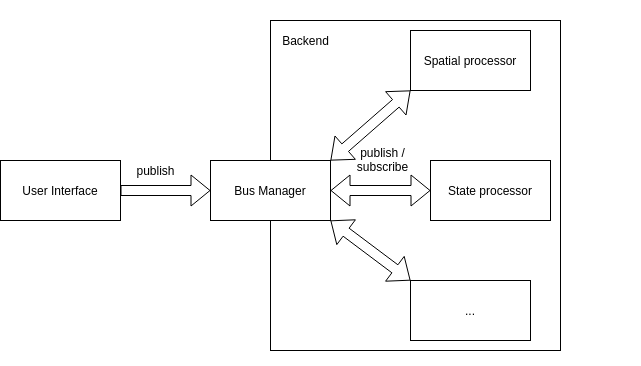
\includegraphics[width=.6\linewidth]{images/couchedit-processors}
  \caption{Publish Subscribe architecture of CouchEdit}
  \label{fig:processors}
\end{figure}

Some of these processors are needed for every type of syntax model, for example the spatial processor, that processes how nodes in the concrete syntax are positioned to each other (above, besides, etc.). Other processors are specific to the given modeling syntax, for example a state chart syntax would require a state processor, that processes if a given graphical object represents a state (usually true if the given node is a rectangle with rounded edges).

A modeling syntax parser for CouchEdit would has to generate these syntax specific processors, while considering multiple design constraints that result from this architecture. Thus a metamodel is needed that can define the desired abstract modeling syntax and specify how a concrete graphical syntax can be mapped to this abstract syntax. While there is ongoing research in the area of relaxed conformance editing and how to link concrete and abstract syntax, it does not immediately become clear what such a metamodel can look like.

\section{Purpose of this Study}
The primary purpose of this study was to develop a metamodel for the CouchEdit framework. This metamodel is supposed to provide a comprehensive and easy to use way for defining new modeling languages. To evaluate the applicability of this metamodel, furthermore a prototypical code generator was implemented, that can comprehend this newly designed metamodel and translate it into a source code implementation.

This extension of the CouchEdit framework is supposed to improve developer accessibility and framework flexibility. While a code generator means that the system still has to be recompiled for every modeling syntax, it still becomes easier to support new modeling syntaxes as the metamodel abstracts away from the actual source code implementation and thus requires less knowledge about the CouchEdit framework.


\section{Research Questions}
\comment{rewrite to fit thesis}

The primary goal of this research will be the development of a metamodel for the CouchEdit framework. This imposes multiple questions which are to be answered in order to design and evaluate the designated metamodel.

\begin{description}
  \item[RQ1:] Is it possible to define a concise metamodel that covers CouchEdits complete feature set?

        If this is not possible, the following question has to be answered.
        \begin{description}
          \item[RQ1.1:] How could the feature set be narrowed down, without impacting the frameworks capabilities too much?
        \end{description}

  \item[RQ2:] What requirements does the CouchEdit architecture impose onto a metamodel?

        The architectures characteristics and quirks have to be considered when designing the language. For example, the publish and subscribe pattern, could make it easy to introduce nonterminating processing chains, which the metamodel should prevent where possible.

  \item[RQ3:] How applicable is the designed metamodel for defining new modeling syntaxes?

        \begin{description}
          \item[RQ3.1] Is it possible to express common modeling syntax concepts in a clear and concise way?
          \item[RQ3.2] Are complex concepts still expressible without causing to much convolution?
        \end{description}
\end{description}


\section{Methodology}
\comment{also only pasted right now}

As this research strives to develop a new metamodel suitable for the CouchEdit framework, it will be conducted in accordance to the Design Science Research (DSR) approach. According to V. Vaishnavi et al. a design science research process consists of five steps \cite{Vaishnavi2004}.

\subsection{Problem Awareness}
The first step of a design science research is the identification of existing problems. As specified in section \ref{sec:problem_statement}, it was identified that the current CouchEdit implementation lacks an user friendly way of adapting it to different modeling syntaxes and that it is unclear how a metamodel for this architecture would look like.

\subsection{Suggestion}
With a clear definition of the problem, objectives can be proposed which have to be achieved in order to solve this problem. The first objective of this research is to develop a metamodel for the CouchEdit architecture. To be more precise, a metamodel is to be designed, that can be used to specify model syntax definitions which map concrete graphical syntaxes to Abstract syntax models and is applicable to CouchEdit's architecture. The second objective is to implement a prototype that provides proof of concept for the applicability of the design metamodel.


\subsection{Development}
The primary goal of a design science research is the development of artifacts.
The first artifact to be developed in this research will be a metamodel, that can be used to define new modeling syntaxes for a relaxed conformance editor and is applicable to CouchEdit's architecture. The second artifact that is to be developed, is a prototypical code generator that can translate the developed metamodel into a CouchEdit implementation which will be able to process the defined modeling syntax.

To this end, the first sub step of the development stage will be to do a comprehensive analysis of CouchEdits architecture. In his work L. Nachreiner describes in detail, which modeling features the framework covers and how they are implemented \cite{nachreiner_couchedit_2020}. For each of these features, a sub metamodel has to be designed that can be used to define the given feature (RQ1). The approaches of \cite{minas_specifying_2001} and \cite{fondement_making_2005} provide a DSL implementation from which concepts for potential metamodels could be derived. If for one of the features, a suitable metamodel cannot be found, it would have to be evaluated if the feature could be simplified or even dropped (R1.1). After designing sub metamodels for all features, they then have to be composed together, which results in a first version of an applicable metamodel. 

in the next sub step, the code generator will be implemented, this is an iterative step. first, an implementation will be developed on the basis of the designed metamodel, this should reveal further requirements imposed by CouchEdits architecture (RQ2). The metamodel then has to be adjusted to account for these requirements, which in turn requires changes of the implementation until no further requirements can be deduced. Because of time constraints it will not be possible to implement all of the metamodel's features, instead the prototype will cover a minimal feature set that still suffices to demonstrate the metamodel's applicability for selected modeling syntaxes.

\subsection{Evaluation}
Now that the desired artifacts are fully developed it has to be evaluated how well they do their designated task. The metamodel as the primary artifact of this research has to be evaluated in terms of its applicability to its designated domain. To this end, the metamodel will be demonstrated on the basis of different modeling syntaxes, this should highlight areas in which the metamodel's design excels, as well as design flaws and limitations (RQ3). If time allows, potential flaws can be addressed by returning back to the development phase and revising the artifacts, otherwise flaws are to be highlighted so that future works can address them.

\subsection{Conclusion}
The conclusion stage marks the end of a DSR and the results are written up. This works written part will be the resulting bachelor's thesis as well as all source code and documentation.


\section{Limitations}
\comment{\dots}
\begin{itemize}
  \item not a complete metamodel designed. common language concepts ignored
\end{itemize}

\section{Thesis Structure}
\comment{\dots}
\section{Problem Statement}

A general purpose framework should be configurable for multiple use cases in its designated domain. CouchEdit as a general purpose graphical modeling framework thus should be configurable for multiple modeling syntaxes. Technically this is possible, as long as one has access to the source code. But this would mean, every time CouchEdit has to support a new modeling syntax, manual changes in the source code have to be made and the project has to be compiled from sources. The implementation of a configuration parser, that can interpret modelling syntax definitions at runtime would thus increase flexibility. Furthermore a well designed metamodel could reduce the amount of knowledge that is needed about the CouchEdit framework.

As a relaxed conformance editing framework, CouchEdit poses special architectural requirements. It has to allow for temporary inconsistencies between concrete syntax (what the user draws) and abstract syntax (what the underlying Model actually looks like). As the concrete syntax does not always have to map to a syntactic correct abstract model, this allows for more freedom in the modeling process (e.g. dangling transitions).

CouchEdit achieves this by building upon the architecture concept of clear separation between concrete and abstract syntax, proposed by Y. Van Tendeloo et al. \cite{van_tendeloo_concrete_2017}. Internally, CouchEdit builds a hypergraph, that maps the given concrete syntax to all possible abstract syntaxes (interpretation of a concrete syntax can be ambiguous and thus multiple abstract syntaxes can be possible). To build this Hypergraph, a set of Processors is employed, which are connected in a reactive publish and subscribe pattern. All Processors (and the user interface) are subscribed to a bus (fig. \ref{fig:processors}). If a change (diff) is published to the bus (e.g. the user adds a node to the concrete syntax), all processors that are subscribed to this type of diff are notified and calculate new resulting diffs, these new diffs are then also published to the bus and all processors interested in them are invoked as well.

\begin{figure}
  \centering
  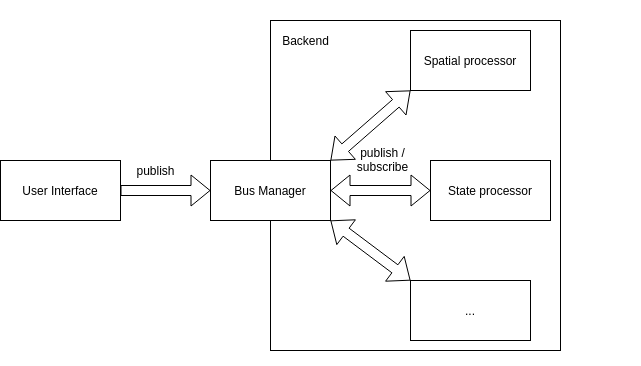
\includegraphics[width=.6\linewidth]{images/couchedit-processors}
  \caption{Publish Subscribe architecture of CouchEdit}
  \label{fig:processors}
\end{figure}

Some of these processors are needed for every type of syntax model, for example the spatial processor, that processes how nodes in the concrete syntax are positioned to each other (above, besides, etc.). Other processors are specific to the given modeling syntax, for example a state chart syntax would require a state processor, that processes if a given graphical object represents a state (usually true if the given node is a rectangle with rounded edges).

A modeling syntax parser for CouchEdit would have to generate these syntax specific processors, while considering multiple design constraints that result from this architecture. Thus a metamodel is needed that can define the desired abstract modeling syntax and specify how a concrete graphical syntax can be mapped to this abstract syntax. While there is ongoing research in the area of relaxed conformance editing and how to link concrete and abstract syntax, it does not immediately become clear what such a metamodel would look like.

\section{Purpose of this Study}
The primary purpose of this study was to develop a metamodel for the CouchEdit framework. This metamodel is supposed to provide a comprehensive and easy to use way for defining new modeling languages. To evaluate the applicability of this metamodel, furthermore a prototypical code generator was implemented, that can comprehend this newly designed metamodel and translate it into a source code implementation.

This extension of the CouchEdit framework is supposed to improve developer accessibility and framework flexibility. While a code generator means that the system still has to be recompiled for every modeling syntax, it still becomes easier to support new modeling syntaxes as the metamodel abstracts away from the actual source code implementation and thus requires less knowledge about the CouchEdit framework.
\chapter{Evaluation}
\label{ch:evaluation}
One of the most important parts of a Design Science Research process is the evaluation. The developed artifact has to be analyzed and it has to be established, how well the defined goals are realized by the artifact.

The main criteria that has to be evaluated, is the applicability of the developed artifact. Meaning, it has to be analyzed how well the developed artifact satisfies the defined goal. To this end it seems worthwhile to evaluate the prototypes performance as well as its developer usability.

\section{Performance}
\label{sec:performance}
To provide performance optimization possibilities, \textsc{CouchEdit} was developed with the \emph{Diff} system in mind. Diffs provide the possibility to calculate changes, without the need for reevaluating the complete hypergraph. On the flipside, this means that all possible states of the graph have to be minded. Using this Diff based approach was evaluated as laborious and error prone, but proved invaluable to improve performance of certain processing tasks \cite{nachreiner_couchedit_2020}. Nachreiner's test results showed that especially language specific processing tasks only took up a small amount of the complete processing time. On basis of this result it was decided, that the developed artifact, primarily concerned with language processing, can produce components that reevaluate the complete graph on every change. Plugin processors, such as the LabelProcessor that is expected to cause high load, are still implemented on application level and thus can make use of the performance benefits granted by the Diff system.

While this research can not produce thorough performance results, it was nonetheless attempted to provide a simple indication of the artifact's impact on performance. To this end the \texttt{StateGridTest} defined in \cite{nachreiner_couchedit_2020} (\Cref{app:testsetup}) was adapted to work with the code generated by the Statecharts implementation (\Cref{sec:state-impl}). The StateGridTest was then run 50 times for both the reference implementation of \cite{nachreiner_couchedit_2020} and the implementation of \Cref{sec:state-impl}. The tests were carried out on a modern system containing an Intel Xeon E2-1231 v3 CPU with 3.40GHz clock an 16GB DDR3 RAM with 1600MHz clock. the system was running windows 10 version 2004. The results of this test suit are depicted in \Cref{fig:performance}. It becomes immediately clear that the generated code performs worse than the reference implementation. especially with higher counts of GraphicObjects the generated implementation needs exponentially more time then the reference values. During test runs it became clear that the generated implementation starts to max out CPU capacity very early on. Thus the rapid growth in processing time can be attributed to hardware bottlenecks. 

\begin{figure}
  \centering
  \begin{tikzpicture}
    \begin{axis}[
        width=.8\linewidth,
        height=7cm,
        ylabel={Processing time in ms},
        xlabel={Number of States},
        xtick={1,2,3,4,5,6,7,8,9,10,11},
        xticklabels={9,16,25,36,49,64,81,100,121,144,169}
      ]
      \addplot table [x=a, y=b, col sep=comma] {generatedimpl.csv};
      \addlegendentry{generated}
      \addplot table [x=a, y=b, col sep=comma] {nativeimpl.csv};
      \addlegendentry{native}
    \end{axis}
  \end{tikzpicture}
  \caption{Performance comparison between reference implementation and generated implementation in the StateGridTest}
  \label{fig:performance}
\end{figure}

While the exact culprit responsible for this rapid growth of processing time is not immediately clear, there are still multiple points that could attribute to this bad performance. First an foremost reevaluating the complete hypergraph in the current implementation is probably the biggest contributor to processing time. In the undirected architecture of \textsc{CouchEdit}, publishing a single change to the hypergraph means that every processor interested in this change will be triggered. The current implementation of the code generator is not able to prune the elements a processor is interested in. This would require analysis of constraints and rules, which requires a complete metamodel definition of this part. Therefore every change published triggers all processors no matter if they are interested in the type of change. This, combined with the fact that each generated processor reevaluates the complete state causes a lot of overhead. Future implementations could try to amend this problem by introducing the aforementioned constraint and rule analysis and use it to prune the hypergraph of each processor. Furthermore it could be possible to reintroduce the Diff based architecture into generated processors. This requires that it is possible to determine which parts of the hypergraph are actually affected by a given Diff. lastly, the developed metamodel introduces a more structured ordering of processors. This could be used to split up processors into sub groups. This way processors in the same group will calculate changes until no processor can produce new changes. All changes calculated are then bundled and passed to the next group. This could reduce the number of times a generated processor is triggered and has to reevaluate the state.

\begin{figure}
  \centering
  \includesvg[width=\linewidth]{images/"component - sub-groups"}
  \caption{\texttt{Processors} split into subgroups, where one group is only activated if the previous group has finished processing.}
  \label{fig:sub-groups}
\end{figure}

\section{Usability}
Developer usability ask the question on how easy it is to use a tool. The main focus of this research was to develop an artifact that simplifies the process of implementing new modeling syntax configurations for \textsc{CouchEdit}. To this end, it has to be evaluated how well the developed artifact achieves this goal. To find a comprehensive answer to this question, a user study is required. Given the state of the developed artifact as well as the time required to conduct a survey, this goes far beyond the projects scope. Therefore, alternative metrics have to be dissected, in order to determine an inclination regarding this question.

One metric to highlight is conciseness. As an abstraction of the \textsc{CouchEdit} architecture, the developed artifact should be able to implement similar concepts in less lines of code. The example implementations reflect this. The Petrinets implementation is \petriConfigLoC lines long and produces \petriGeneratedLoC lines of code. Equally, the Statecharts implementation consists of \stateConfigLoC and generates \stateGeneratedLoC lines. In both examples, this means, on average of over 6 lines of source code are generated per line of the configuration. Of course, the code generator most likely generates code that is more verbose than an equivalent written by a developer. therefore this metric is flawed and only serves as a suggestion for the possible usability.

To further reinforce claims of conciseness, the Statecharts example (\Cref{sec:state-impl}) was modeled as closely as possible after the Statecharts configuration implemented in \cite{nachreiner_couchedit_2020}. An exact replica of the modeling syntax implemented by Nachreiner is not possible. The abstract syntax metamodel defined by them, utilizes \texttt{Relations}, which the AbstractMM defined in \Cref{sec:abstract-syntax} does not support. This results from the close orientation towards Ecore. Furthermore, the \texttt{ConcreteMM} is opinionated in its approach to define configurations and thus, can naturally not provide the same flexibility as an application level implementation has. Nonetheless, the application level implementation is 1900 lines long \cite{nachreiner_couchedit_2020}, and was realized here in \stateConfigLoC lines. This is primarily contributed to the fact that implementations using the metamodel do not have to mind every possible state of the graph, as well as the reduction of a lot of boilerplate code.

While the artifact abstracts away from the implementation details of \texttt{Processors}, the developer still requires certain knowledge about the framework. Most prominently a developer has to understand the hypergraph. Constraints and rules usually require querying of the hypergraph, therefore it is inevitable to know the existing element types as well as possible Relations and their meaning. Furthermore, it has to be understood which changes, different plugins apply to the graph, as well as what functions are available. Nonetheless, the amount of knowledge required, is still reduced.

\subsection{plugins}
The plugin system proved as a worthwhile addition to the architecture. The example language configurations, described in \Cref{sec:example-configs} show of how complex tasks can be trivialized if the correct plugin is provided. With the plugin system, new \texttt{Processors} can be added to the library of existing processors, should problems arise that are difficult to solve within the generalized metamodel architecture. Plugins are developed on the application level an thus have access to \textsc{CouchEdit}'s complete architecture. On the other hand, this means that developing plugins requires knowledge over the complete \textsc{CouchEdit} framework, which the developed artifact is trying to abstract. Therefore plugins should be implemented as general as possible, so that they can be reused as much as possible. Therein lies the challenge of the plugin system. The usefulness of a plugin depends on how well it can be adapted to different modeling syntaxes. This means that plugins have to be developed with great care. In the example Statecharts implementation (\Cref{sec:state-impl}), the \texttt{LabelProcessor} prototype failed to solve all labeling requirements imposed by the syntax. This demonstrates the volatility of hastily developed plugin. On the other hand, the ConnectionPlugin, thanks to its simplicity was able to provide a concise solution for the given problem.

\section{Discussion of DisplayClasses}
\label{sec:dc-disc}
During initial evaluation of the architecture proposed by Fondement and Baar \cite{fondement_making_2005} it was decided to not adapt the concept of \texttt{DisplayClasses}, proposed by the Authors. This decision was made, because their implementation details were not certain. It was estimated, that \texttt{DisplayClasses} would introduce further complexity without providing any significant advantages. with regards to the developed artifact, this turned out as mostly true. Nonetheless, there are certain scenarios as well as considerations towards future work that could make an implementation utilizing \texttt{DisplayClasses} relevant.

When tightening requirements towards the concrete syntax DisplayClasses could prove useful. For example, if it is required that a Place in the Petrinets syntax always has a name, the same part of the graph has to be queried two times. First the PlacePatternProcessor would have to check if a label is assigned to a Place before it can add the Pattern element of type Place. Then the PlaceRecognitionProcessor can add the PlaceDM. Afterwards the PlaceSyncProcessor has to query the same part of the Graph that the PlacePatternProcessor already queried, to find the corresponding label. Using DisplayClasses, this double querying could be prevented, as the PlaceSyncProcessor would have to just get the Label that is connected to the DisplayClass already, similar to the invariant shown in \Cref{lst:ocl-inv}.


Another scenario that could make \texttt{DisplayClasses} relevant is concerned with syntax feedback in the frontend. \textsc{DiaGen} marks graphical element in a different color, if they are part of a syntactic correct concrete representation \cite{minas_concepts_2002}. Such a feature could be conceivable in future iterations of frontends for \textsc{CouchEdit}. With the pattern system developed in this thesis, there does not exist a direct connection between all \texttt{GOs} and the abstract representation they are part of. Using \texttt{DisplayClasses}, every \texttt{GO} has a direct connection to the abstract representation they are mapped to. Thus, \texttt{DisplayClasses} would trivialize implementation of a feature similar to \textsc{DiaGen}'s.


% \begin{itemize}
%   \item suggestions
%   \item syntactic correctness
%   \item plugin processor needed for specialized tasks
%   \item plugins need to to be well designed (to specialized\\
%         and is general applicability drops,badly designed config model and its a hassle to use )
% \end{itemize}


\chapter{Conclusion}
\label{ch:conclusion}

This work presented an experimental architecture that can be used to define modeling syntax configurations for \textsc{CouchEdit}. To this end, the approach of Fondement and Baar \cite{fondement_making_2005} was adapted and extended to fit the needs of the \textsc{CouchEdit} architecture. Their approach is composed of two parts, recognition and synchronization. These two mechanisms were integrated into the developed artifact as the core concept. This concept was then extended by a plugin system, which allows for modular components that can be configured to satisfy different modeling syntaxes' requirements.

It was shown that the developed artifact seems applicable for the task of specifying modeling syntaxes for \textsc{CouchEdit}. However, while it is possible to define modeling syntaxes, especially the definition of well designed Plugins is key to general applicability and developer experience. Furthermore, performance test results indicate that the developed artifact in its current iteration produces configurations that increase processing overhead tenfold compared to a Diff-based implementation on the application-level.  

\section{Future Work}
This research poses a set of new questions that have to be answered. First and foremost, it has to be evaluated if the system's performance can be improved to reach acceptable levels. Towards this goal, multiple mechanisms could be researched.

One of the next major iterations of this artifact would be to develop a complete DSL implementation. This would allow for multiple optimizations. First, the hypergraph each processor requires could be pruned to contain only the elements relevant to a given processor. in its current iteration the code generator has no information about the defined constraints and rules, this means that each processor has to be configured to potentially use all possible elements of the hypergraph. therefore processors are triggered even when changes are published that have no importance for them. Furthermore, it could be researched if the extra information given by a complete metamodel definition can be utilized to generate processors using ModelDiffs. The results provided in \Cref{sec:performance} indicate that evaluation of the complete hypergraph does not scale well. If it is possible to reevaluate only parts of the hypergraph that are actually affected by incoming changes, this could improve performance considerably.

The plugin system proved to be a critical mechanism for the applicability of the developed metamodel. Plugins can take up many tasks from the user and bring further performance improvements as they are implemented on the application-level. Therefore, they can make use of the available optimization schemes. Nevertheless, \Cref{sec:state-impl} showed that a plugin's design is crucial to ensure the applicability for a wide range of modeling syntaxes. Thus it has to be evaluated which plugins are needed and how they could be implemented. The LabelPlugin was shown off as a Plugin that is integral to many Modeling languages and thus has to receive further attention to reach its full potential. Moreover, the CompartmentPlugin, as well as the ConnectionPlugin, could receive further improvements by introducing configuration possibilities. Besides the existing Plugins, it also seems worthwhile to further investigate mechanisms that could be implemented as Plugins. To this end, the works of \cite{van_tendeloo_concrete_2017} and \cite{costagliola_classification_2002} could provide a basis to build upon. 

It is also essential to investigate the artifact's applicability towards correctness checking. It is critical for editor usability to convey to the user if the designed concrete model can be mapped to a correct abstract representation. To this end, it was evaluated that the introduction of DisplayClasses could result in a more explicit connection of abstract and concrete syntax and thus make it easy to decide which graphic objects art part of an abstract representation. Additionally, the work of Baar \cite{baar_correctly_2008} could be used as a foundation to introduce correctness checking into the framework.

Distributed modeling is one of the potential applications of \textsc{CouchEdit}, which means development using multiple frontends that only share an abstract representation. For this to be possible, the architecture has to be able to translate from abstract to concrete syntax. In its current Iteration, the architecture is not able to do this. The artifact generates processors that strictly translate from concrete to abstract syntax. Therefore it has to be evaluated if it is possible to introduce bidirectionality into the prototype. 


An critical concept theorized for the \textsc{CouchEdit} framework is the general model action mechanism \cite{nachreiner_couchedit_2020}. In the form of \emph{Suggestions}, they can provide the user with options that can be used to disambiguate the hypergraph or provide quick fixes that give the user fast actions to transform a malformed graph into something correct. The developed artifact currently does not support any functionality for model actions. To this end, further research is needed to find out how this functionality could integrate with the system.

In the early stages of this research, it was decided to use the approach proposed by Fondement and Baar \cite{fondement_making_2005}. Developing an alternative architecture that builds upon TGGs could bring multiple benefits. Especially the bidirectionality would bring advantages in regards to the future of this project While the incremental 


% \begin{description}
%   \item[Plugin System]
%   \item[Suggestions] 
%   \item[Perceptualization]  
% \end{description}

% \begin{itemize}
%   \item develop functional DSL
%   \item check performance loss
%   \item usability test especially in terms of complex graphic objects
%   \item abstract syntax correctness and feedback to user
% \end{itemize}






















% Abbildungsverzeichnis
\cleardoublepage % sonst stimmt die seitennummer im TOC nicht
\phantomsection
\addcontentsline{toc}{chapter}{Abbildungsverzeichnis}
\listoffigures


% Tabellenverzeichnis
\cleardoublepage % sonst stimmt die seitennummer im TOC nicht
\phantomsection
\addcontentsline{toc}{chapter}{Tabellenverzeichnis}
\listoftables


% Bibliographie (am besten mit Bibtex oder Biber)
\cleardoublepage % sonst stimmt die seitennummer im TOC nicht
\phantomsection
\addcontentsline{toc}{chapter}{Literaturverzeichnis}
\printbibliography

% Declaration of Independance
\clearpage
\thispagestyle{empty}

\noindent Name: \fullname \hfill Matrikelnummer: \matrikelnummer \vspace{2cm}

\minisec{Erklärung}

Ich erkläre, dass ich die Arbeit selbständig verfasst und keine anderen als die angegebenen Quellen und Hilfsmittel verwendet habe.\vspace{2cm}

\noindent Ulm, den \dotfill

\hspace{10cm} {\footnotesize \fullname}





\end{document}
